\documentclass[11pt]{article}
\usepackage[T1]{fontenc}
\usepackage{amsmath,amssymb,amsthm,mathtools,booktabs,geometry,graphicx,enumitem}
\usepackage[hidelinks]{hyperref}
\geometry{margin=1in}
\setlength{\emergencystretch}{2em}
\allowdisplaybreaks

\newtheorem{theorem}{Theorem}[section]
\newtheorem{proposition}[theorem]{Proposition}
\newtheorem{lemma}[theorem]{Lemma}
\newtheorem{corollary}[theorem]{Corollary}
\theoremstyle{definition}
\newtheorem{definition}[theorem]{Definition}
\newtheorem{assumption}[theorem]{Assumption}
\theoremstyle{remark}
\newtheorem{remark}[theorem]{Remark}

\newcommand{\R}{\mathbb R}
\newcommand{\E}{\mathbb E}
\newcommand{\Var}{\operatorname{Var}}
\newcommand{\He}{\mathrm{He}}
\newcommand{\repo}{\url{https://github.com/RamanJamal1/gcm-logconcave-counterexamples}}

\title{Signs of Entropy Derivatives along the Heat Flow for Log-Concave Densities:
Exact Certificates through Order Thirteen and a Counterexample at Order Sixteen}
\author{Raman Jamal\thanks{ORCID: \href{https://orcid.org/0009-0004-7042-8149}{0009-0004-7042-8149}.}}
\date{Version 0.2.0, November 2026}

\begin{document}
\maketitle

\begin{abstract}
For a probability density $p$ on the real line let $P_t$ denote the heat semigroup
and $H(p)=\int p\log p$ the Boltzmann entropy, and set
$S_m(p)=(-1)^m\partial_t^mH(P_tp)|_{t=0}$. The Gaussian completely monotone
conjecture asserts $S_m\ge0$ for every $m$. It is false for general densities, and
it is known to fail also for log-concave densities, but only at an unspecified order
or at all sufficiently large orders. We study the first failing order
$m^*=\min\{m:\ S_m(p)<0\text{ for some log-concave }p\}$. An exact rational
sum-of-squares identity at order thirteen, checked by a standalone exact verifier,
together with a propagation argument along the heat flow, shows that
$S_m(P_tp)\ge0$ for every log-concave density $p$, every $t>0$ and every $m\le13$,
and $S_m(p)\ge0$ under an endpoint-regularity assumption. Sharper identities give
McKean's Gaussian optimality bound $S_m(p)\Var(p)^m\ge(m-1)!/2$ for log-concave
densities at every order $m\le11$, extending the previously known range $m\le5$. An explicit
log-concave density with three Fourier modes has $S_{16}<-3/4$, certified by two
independent interval-arithmetic computations. Hence $14\le m^*\le16$. We also show
that the explicit family of Zou, Fan, Gao and Wang first fails at order $33$.
The value of $m^*$ within the bracket remains open.
\end{abstract}

\noindent\textbf{Keywords:} entropy, heat flow, Fisher information, log-concave
density, completely monotone conjecture, sum of squares, computer-assisted proof,
interval arithmetic.

\noindent\textbf{MSC 2020:} 94A17, 60E15, 35K05, 90C22, 65G20.

\section{Introduction}

\subsection{Background}
Let $X$ be a real random variable with density $p$, and let $Z$ be an independent
standard Gaussian. The density of $X+\sqrt tZ$ is $P_tp$, where
$P_t=e^{t\partial_x^2/2}$ is the heat semigroup with generator $\tfrac12\partial_x^2$.
Throughout we use the Boltzmann entropy
\[
 H(p)=\int_\R p\log p,
\]
which is the negative of the differential (Shannon) entropy; all signs below reverse
under the other convention. De Bruijn's identity~\cite{Stam59} gives
$\partial_tH(P_tp)=-\tfrac12I(P_tp)$, where $I$ is the Fisher information, and
Costa's concavity of the entropy power~\cite{Costa85} concerns the second derivative.
McKean~\cite{McKean66} studied the signs of the higher derivatives in the context of
Kac's model, and Cheng and Geng~\cite{ChengGeng15} formulated the
\emph{Gaussian completely monotone conjecture}: with
\[
 S_m(p)=(-1)^m\left.\partial_t^mH(P_tp)\right|_{t=0},
\]
one has $S_m(p)\ge0$ for all $m\ge1$, i.e.\ $t\mapsto -\partial_tH(P_tp)$ is
completely monotone. Cheng and Geng verified it in dimension one through order four.
McKean~\cite{McKean66} also conjectured that, among densities with a given variance,
the Gaussian minimizes each $S_m$ (McKean's \emph{Gaussian optimality conjecture}).
Zhang, Anantharam and Geng~\cite{ZAG18} reduced such statements to linear matrix
inequalities and proved that McKean's conjecture holds for orders up to five when the
density of $X+\sqrt tZ$ is log-concave, which is the case when $p$ is log-concave;
Wang~\cite{Wang24} proved the sign condition through order five for log-concave
inputs in every dimension by a higher-order Otto calculus. See also~\cite{GYG22} for
multivariate higher-order derivatives.

Gu and Sellke~\cite{GuSellke26} disproved the conjecture, and with it McKean's Gaussian
optimality conjecture: an explicit discrete measure gives a negative fifth derivative
at a positive time. For log-concave inputs the signs are known through order
five~\cite{ZAG18,Wang24}, and Gu and Sellke showed, by a backward-propagation argument,
that the conjecture nevertheless fails for some log-concave density at some
\emph{unspecified} order. Zou, Fan, Gao and Wang~\cite{ZFGW26} constructed an explicit
log-concave family $f_m$ with $S_m(f_m)<0$ for all \emph{sufficiently large} $m$,
without an explicit threshold; for dimension $d\ge2$ see also~\cite{ZFGW26hex}. This
leaves the natural question
\[
 m^*:=\min\{m\ge1:\ S_m(p)<0\ \text{for some log-concave probability density }p\},
\]
where only densities for which $S_m(p)$ is defined are considered (see
Assumption~\ref{ass:endpoint} and Remark~\ref{rem:positive-times}). The results above
give $m^*\ge6$.

\subsection{Main results}
Denote by $\mathcal{LC}$ the smooth, strictly positive, log-concave probability
densities on $\R$. Since $S_m(p)$ is a derivative at the endpoint $t=0$, we make the
following convention explicit.

\begin{assumption}[Endpoint regularity]\label{ass:endpoint}
For $p\in\mathcal{LC}$ and a given order $m$, the function $t\mapsto H(P_tp)$ admits
an order-$m$ right Taylor expansion at $t=0$; $S_m(p)$ denotes the corresponding
signed right derivative.
\end{assumption}

\begin{remark}[Positive times]\label{rem:positive-times}
For $t>0$ the density $P_tp$ is smooth, strictly positive and log-concave,
$s\mapsto H(P_sp)$ is $C^\infty$ on $(0,\infty)$ (Lemma~\ref{lem:positive}), and
$S_m(P_tp)$ is the signed $m$-th derivative of $s\mapsto H(P_sp)$ at $s=t$. A sign
failure at a positive time is therefore a failure at time zero for the log-concave
density $P_tp$, and $m^*$ is unchanged if positive times are allowed. The
order-sixteen witness of Section~\ref{sec:witness} satisfies
Assumption~\ref{ass:endpoint}: its heat evolution is explicit for small $|t|$, and
$t\mapsto H(P_tp_{16})$ is $C^\infty$ near $t=0$ by differentiation under the
integral sign.
\end{remark}

\begin{theorem}[Certified bracket]\label{thm:main}
\begin{enumerate}[label=(\roman*)]
\item For every log-concave probability density $p$ (not necessarily smooth), every
 $t>0$ and every $1\le m\le13$, $S_m(P_tp)\ge0$; the orders $m\le5$ were
 known~\cite{ZAG18,Wang24}. If $p\in\mathcal{LC}$ satisfies
 Assumption~\ref{ass:endpoint} at order $m$, then also $S_m(p)\ge0$.
\item The density
 \[
 p_{16}(x)=Z^{-1}e^{-x^2/28}\Bigl(1+\tfrac{\cos x}{15}+\tfrac{\cos2x}{40000}
 -\tfrac{\cos3x}{18000000}\Bigr),
 \]
 with the explicit normalizer of Proposition~\ref{prop:witness}, satisfies
 $(-\log p_{16})''\ge 25777/235206314>10^{-4}$ on $\R$ and $S_{16}(p_{16})<-3/4$.
\end{enumerate}
Consequently $14\le m^*\le16$.
\end{theorem}

\begin{theorem}[Gaussian optimality for log-concave densities]\label{thm:sharp}
Let $p$ be a log-concave probability density with variance $v$, and let
$1\le m\le11$. Then for every $t>0$
\[
 S_m(P_tp)\,(v+t)^m\ \ge\ \frac{(m-1)!}{2},
\]
with equality if and only if $p$ is Gaussian. If $p\in\mathcal{LC}$ satisfies
Assumption~\ref{ass:endpoint} at order $m$, then $S_m(p)\,v^m\ge(m-1)!/2$. In
particular $S_6v^6\ge60$, $S_7v^7\ge360$ and $S_8v^8\ge2520$. This is McKean's
Gaussian optimality conjecture for log-concave densities at orders $m\le11$; for
$m\le5$ it was proved in~\cite{ZAG18}.
\end{theorem}

\begin{remark}[Equality at $t=0$]\label{rem:equality-endpoint}
The endpoint argument of Section~\ref{sec:endpoint} transfers the inequality of
Theorem~\ref{thm:sharp} to $t=0$ but not the characterization of equality, since a
strict inequality at every $t>0$ may become an equality in the limit. Equality at
$t=0$ forces $p$ to be Gaussian whenever the representation $S_m(p)=(-1)^m\E_pF_m$
and the identities~\eqref{eq:ibp} hold for $p$ itself, for instance under the
hypotheses of Proposition~\ref{prop:recurrence}.
\end{remark}

\begin{theorem}[The Zou--Fan--Gao--Wang family]\label{thm:zou}
Let $f_M\propto e^{-\kappa_Mx^2/2}(1+a_M\cos x+b_M\cos2x)$ with $a_M=2^{-M/4}$,
$b_M=2^{-M}$ and $\kappa_M=8a_M$. Then $S_M(f_M)>0$ for $6\le M\le32$ and
$S_M(f_M)<0$ for $33\le M\le400$. Since $S_M\ge0$ for every log-concave density when
$M\le5$~\cite{ZAG18,Wang24}, the first order at which the family violates the sign
condition is $33$.
\end{theorem}

\subsection{Nature of the proofs}
Theorem~\ref{thm:main}(i) and Theorem~\ref{thm:sharp} rest on explicit polynomial
identities in the jet variables $u_j=\partial_x^j\log p$, with rational positive
definite Gram matrices (Section~\ref{sec:sos}). Each identity is checked by a
standalone verifier written in the Python standard library, separate from the search
and reconstruction code (all of the code was produced in the same AI-assisted
workflow; see the statement on the use of AI), which re-derives the
entropy polynomial independently and verifies positivity by exact rational Schur
complements; no floating-point solver output is used as evidence. Theorem~\ref{thm:main}(ii)
and Theorem~\ref{thm:zou} rest on outward-rounded ball arithmetic
(Arb~\cite{Johansson17}) with analytic bounds for all truncated tails.

\begin{remark}[What is machine-checked]\label{rem:status}
The computer verifies (a) the polynomial identities and the positive definiteness of
the Gram matrices, (b) the global curvature bound for $p_{16}$, and (c) the interval
enclosures of the entropy derivatives. The passage from an identity to an inequality
for every log-concave density uses the analytic arguments of
Lemma~\ref{lem:positive} and Sections~\ref{sec:positive-time}--\ref{sec:sharp-proof}
(positive-time regularity, the endpoint argument, downward propagation and the proof
of Theorem~\ref{thm:sharp}). These are written arguments, not machine-checked, and
they are the parts of the paper on which expert scrutiny is most needed.
\end{remark}

\subsection{Organization}
Section~\ref{sec:prelim} fixes notation and derives the reduced integrands.
Section~\ref{sec:sos} states the certificate form and derives the sign consequences,
including the propagation lemma and the sharp bounds. Section~\ref{sec:computation}
describes how the certificates were found and verified. Section~\ref{sec:witness}
proves part (ii) of Theorem~\ref{thm:main}, and Section~\ref{sec:zou} proves
Theorem~\ref{thm:zou}. Section~\ref{sec:logcosh} treats a family with exponential
tails, and Section~\ref{sec:discussion} discusses the open orders fourteen and fifteen.
Appendix~\ref{app:formulas} lists reduced integrands and Appendix~\ref{app:series}
the Fourier-series enclosure used in Sections~\ref{sec:witness}--\ref{sec:zou}.

\section{Preliminaries}\label{sec:prelim}

\begin{proposition}[Scaling and Gaussian values]\label{prop:scaling}
For $p_a(x)=a^{-1}p(x/a)$, $a>0$, one has $S_m(p_a)=a^{-2m}S_m(p)$. For the centred
Gaussian of variance $v$, $S_m=(m-1)!/(2v^m)$. Hence $S_m(p)\Var(p)^m$ is scale
invariant, and no strictly positive universal lower bound for unnormalized $S_m$ exists.
\end{proposition}
\begin{proof}
Heat scaling gives $H(P_tp_a)=H(P_{t/a^2}p)-\log a$. For the Gaussian,
$H(P_tp)=-\tfrac12\log(2\pi e(v+t))$. Differentiate $m$ times.
\end{proof}

Write $u_j=\partial_x^j\log p$ and let $D$ be the derivation on polynomials in
$u_1,u_2,\dots$ with $Du_j=u_{j+1}$, so that $\partial_x[P(u(x))]=(DP)(u(x))$.
For a polynomial $P$ and sufficiently regular $p$,
\begin{equation}\label{eq:ibp}
 \int_\R p\,(DP+u_1P)=\int_\R\partial_x(pP)=0 .
\end{equation}
We call $DP+u_1P$ an \emph{integration-by-parts (IBP) identity}. Give $u_j$ weight
$j$; then $\partial_t^mH(P_tp)|_{t=0}$ is the expectation of a polynomial of weighted
degree $2m$.

\begin{proposition}[Reduced derivative recurrence]\label{prop:recurrence}
For smooth densities with Gaussian decay and bounded higher log-derivatives, if $F$
is a polynomial in $u_2,u_3,\dots$ then $\partial_t\E_pF=\E_p\mathcal LF$, where
\[
 \mathcal LF=-\frac12\sum_{i,j\ge2}F_{ij}\,u_{i+1}u_{j+1}
 +\frac12\sum_{i\ge2}F_i\sum_{k=1}^{i-1}\binom ik u_{k+1}u_{i-k+1},
\]
with $F_i=\partial F/\partial u_i$. With $F_2=u_2^2/2$ and $F_m=\mathcal L^{m-2}F_2$
one has $\partial_t^mH(P_tp)|_{t=0}=\E_pF_m$, and $F_m$ involves derivatives of order
at most $m$.
\end{proposition}
\begin{proof}
The heat equation gives $\partial_t\log p=(u_2+u_1^2)/2$. Differentiating $u_i$ in time
produces a diffusion term, a drift term $u_1u_{i+1}$, and the quadratic sum displayed.
Differentiating the expectation contributes $\tfrac12\E_p\partial_x^2F$. Applying
\eqref{eq:ibp} in the form $\E_p(\partial_x^2F+u_1\partial_xF)=0$ eliminates the
drift and combines the second-order terms into $-\tfrac12\sum F_{ij}u_{i+1}u_{j+1}$.
Gaussian tails justify the boundary limits; at positive times
Lemma~\ref{lem:positive} replaces these hypotheses for every log-concave density.
\end{proof}
The integrands $F_6,F_7,F_8$ are listed in Appendix~\ref{app:formulas}. Note that
$S_m(p)=(-1)^m\E_pF_m$.

\section{Sum-of-squares certificates and their consequences}\label{sec:sos}

\subsection{The certificate form}
For $r\ge1$ let $v_r$ be a vector of monomials of weighted degree $r$ in the $u_j$.

\begin{definition}\label{def:cert}
An \emph{order-$m$ certificate} consists of symmetric rational matrices
$Q_0\succ0$, $Q_1\succ0$, rational numbers $\lambda_k$ and monomials $P_k$ of weighted
degree $2m-1$ such that, as polynomials,
\begin{equation}\label{eq:cert}
 (-1)^mF_m=v_m^{\mathsf T}Q_0v_m+(-u_2)\,v_{m-1}^{\mathsf T}Q_1v_{m-1}
 -\sum_k\lambda_k\,(DP_k+u_1P_k).
\end{equation}
A \emph{sharp certificate} replaces the left side by
$(-1)^mF_m-\tfrac12(m-1)!\,(-u_2)^m$, with $v_r$ restricted to monomials containing
at least one $u_j$ with $j\ge3$.
\end{definition}

\begin{proposition}[Sign from a certificate]\label{prop:sign}
Suppose an order-$m$ certificate exists, and let $p\in\mathcal{LC}$ be such that
$S_m(p)=(-1)^m\int pF_m$, every term of \eqref{eq:cert} is $p$-integrable, and
\eqref{eq:ibp} holds for each $P_k$. Then $S_m(p)\ge0$.
\end{proposition}
\begin{proof}
Integrate \eqref{eq:cert} against $p$. The IBP terms vanish. Log-concavity gives
$-u_2\ge0$, and positive definiteness makes both remaining terms pointwise
nonnegative.
\end{proof}

Certificates exist at orders $6,\dots,11$ and $13$, and sharp certificates at orders
$6,\dots,11$ (Table~\ref{tab:certs}).

\subsection{Positive heat times}\label{sec:positive-time}
In this subsection $p$ is an arbitrary log-concave probability density on $\R$ (not
necessarily smooth or positive), $X\sim p$, $Z$ is an independent standard Gaussian,
$t>0$, $Y=X+\sqrt t\,Z$, $p_t=P_tp$ is the density of $Y$, and $u_j=\partial_y^j\log p_t$.

\begin{lemma}[Positive-time regularity]\label{lem:positive}
\begin{enumerate}[label=(\alph*)]
\item $p_t$ is smooth, strictly positive and log-concave.
\item For every $j\ge2$ there is a constant $C_j$ depending only on $j$ such that
 $\sup_y|u_j(y)|\le C_j\,t^{-j/2}$; moreover $-1/t\le u_2\le0$.
\item $\E|u_1(Y)|^q\le t^{-q/2}\,\E|Z|^q$ for every $q\ge1$, and
 $|u_1(y)|\le\bigl(2|y|+|\E[X\mid Y=0]|\bigr)/t$.
\item For every polynomial $P$ in $u_1,u_2,\dots$, the identity~\eqref{eq:ibp} holds
 for $p_t$, all integrands being absolutely integrable.
\item $s\mapsto H(P_sp)$ is $C^\infty$ on $(0,\infty)$ and
 $\partial_s^mH(P_sp)=\E_{p_s}F_m$ for every $m\ge2$, with $F_m$ as in
 Proposition~\ref{prop:recurrence}. In particular $|S_m(P_tp)|\le K_m\,t^{-m}$ with
 $K_m$ depending only on $m$.
\end{enumerate}
\end{lemma}

\begin{proof}
(a) Smoothness and positivity follow from $p_t=p*\varphi_t$, with $\varphi_t$ the
centred Gaussian density of variance $t$; convolution preserves
log-concavity~\cite[Proposition~3.5]{SW14}.

(b) Write $p_t(y)=(2\pi t)^{-1/2}e^{-y^2/(2t)}\int p(x)\,e^{-x^2/(2t)}\,e^{xy/t}\,dx$.
For $j\ge2$ this gives
\[
 u_j(y)=-\frac{\delta_{j2}}{t}+t^{-j}\,\kappa_j(\nu_y),
\]
where $\kappa_j(\nu_y)$ is the $j$-th cumulant of
$\nu_y(dx)\propto p(x)\,e^{-(y-x)^2/(2t)}\,dx$, the conditional law of $X$ given
$Y=y$. For $j=2$ this reads $u_2=-1/t+\Var(\nu_y)/t^2$; since $p_t$ is log-concave,
$u_2\le0$, hence $\Var(\nu_y)\le t$, and trivially $u_2\ge-1/t$. The measure $\nu_y$
is log-concave, and so is the law of $X-m_y$ under $\nu_y$, where
$m_y=\E[X\mid Y=y]$; hence~\cite[Theorem~5.22]{LV07}
$\bigl(\int|x-m_y|^k\,d\nu_y\bigr)^{1/k}\le2k\int|x-m_y|\,d\nu_y\le2k\Var(\nu_y)^{1/2}$.
A cumulant of order $j\ge2$ is a universal polynomial in the central moments of
orders $2,\dots,j$, homogeneous of degree $j$ under scaling, so
$|\kappa_j(\nu_y)|\le C_jt^{j/2}$ uniformly in $y$.

(c) For $k\ge1$,
$p_t^{(k)}(y)/p_t(y)=t^{-k/2}\,\E\bigl[(-1)^k\He_k(Z)\bigm| Y=y\bigr]$, with $\He_k$
the probabilists' Hermite polynomials; the case $k=1$ and conditional Jensen give the
moment bound. Moreover $u_1(y)=(m_y-y)/t$ and $\partial_ym_y=\Var(\nu_y)/t\in[0,1]$,
so $|m_y|\le|m_0|+|y|$.

(d) By (b) and (c), $p_tP$ and $p_t(DP+u_1P)$ are integrable. Let
$\chi\in C_c^\infty(\R)$ equal $1$ near $0$ and $\chi_R(y)=\chi(y/R)$. Then
$\int\chi_R\,p_t(DP+u_1P)=\int\chi_R\,\partial_y(p_tP)=-\int\chi_R'\,p_tP$, whose
modulus is at most $R^{-1}\|\chi'\|_\infty\int p_t|P|\to0$, while the left side tends
to $\int p_t(DP+u_1P)$ by dominated convergence.

(e) Fix $0<t_0<t_1$. A log-concave density has exponential tails,
$p(x)\le Ae^{-a|x|}$, so $p_s(y)\le A\,e^{-a|y|}\,\E\,e^{a\sqrt s|Z|}$ uniformly for
$s\in[t_0,t_1]$; and a bounded set of positive $p$-mass gives
$p_s(y)\ge c\,e^{-by^2}$ there. By (b) and (c), every polynomial in $u_1,u_2,\dots$
(computed for $p_s$) is bounded by $B(1+|y|)^k$ uniformly in $s\in[t_0,t_1]$, since
$s\mapsto\E[X\mid X+\sqrt sZ=0]$ is continuous. The heat equation
$\partial_sp_s=\tfrac12p_s''$ gives $\partial_s\log p_s=\tfrac12(u_2+u_1^2)$ and
$\partial_su_i=\tfrac12u_{i+2}+u_1u_{i+1}+\tfrac12\sum_{k=1}^{i-1}\binom ik
u_{k+1}u_{i-k+1}$, so $\partial_s[p_s\,F(u)]$ is $p_s$ times a polynomial in the $u_j$
and is dominated by an integrable function of $y$ uniformly in $s\in[t_0,t_1]$.
Differentiation under the integral sign is therefore allowed, and the computation in
the proof of Proposition~\ref{prop:recurrence}, in which every integration by parts is
an instance of (d), gives $\partial_s\E_{p_s}F=\E_{p_s}\mathcal LF$. The first
derivative is de Bruijn's identity
$\partial_sH(P_sp)=-\tfrac12\E_{p_s}u_1^2=\tfrac12\E_{p_s}u_2$, justified in the same
way because $|\log p_s(y)|$ grows at most quadratically; and
$\mathcal L(u_2/2)=u_2^2/2=F_2$. Finally $F_m$ is a polynomial in $u_2,\dots,u_m$ of
weighted degree $2m$, so (b) gives $|S_m(P_tp)|\le K_mt^{-m}$.
\end{proof}

Applying Proposition~\ref{prop:sign} to $p_t$, with Lemma~\ref{lem:positive}(d),(e)
supplying its hypotheses, gives $S_m(P_tp)\ge0$ for all $t>0$ at every order with a
certificate.

\subsection{The endpoint}\label{sec:endpoint}
Under Assumption~\ref{ass:endpoint}, continuity and the positive-time sign give
$(-1)^m\Delta_h^mH(P_\cdot p)(0)\ge0$ for the forward differences with step $h>0$;
dividing by $h^m$ and letting $h\downarrow0$ gives $S_m(p)\ge0$. Smoothness of $p$ in
space is not used as a substitute for the existence of the time derivative.

\subsection{Downward propagation}\label{sec:propagation}
\begin{lemma}\label{lem:propagation}
If $S_{r+1}(P_sp)\ge0$ for all $s>0$, then $S_r(P_tp)\ge0$ for all $t>0$.
Consequently a certificate at order $M$ gives the sign at every order $r\le M$.
\end{lemma}
\begin{proof}
By Lemma~\ref{lem:positive}(e), $|S_r(P_tp)|\le K_rt^{-r}$, so $S_r(P_tp)\to0$ as
$t\to\infty$. Since
$\partial_tS_r(P_tp)=-S_{r+1}(P_tp)$,
\[
 S_r(P_tp)=\int_t^\infty S_{r+1}(P_sp)\,ds\ \ge0 .
\]
Induct downward and apply the endpoint argument.
\end{proof}
Applied with $M=13$, Lemma~\ref{lem:propagation} gives the sign at every order
$r\le13$ for all $t>0$, completing Theorem~\ref{thm:main}(i); orders $6$--$11$ and
$13$ also have direct certificates. A sharp variance bound propagates in the same way:
if $S_M(P_sp)\,(v+s)^M\ge(M-1)!/2$ for all $s>0$, then
\begin{align*}
 S_{M-1}(P_tp)&=\int_t^\infty S_M(P_sp)\,ds\\
 &\ge\int_t^\infty\frac{(M-1)!}{2(v+s)^M}\,ds=\frac{(M-2)!}{2(v+t)^{M-1}},
\end{align*}
with equality only if equality holds for almost every $s>t$. Applied with
$M=11,10,\dots$ this yields Theorem~\ref{thm:sharp} at every order $m\le11$ from the
sharp certificate at order $11$; the sharp certificates at orders $6$--$10$ give the
same bounds directly.

\subsection{Sharp bounds}\label{sec:sharp-proof}
\begin{proof}[Proof of Theorem~\ref{thm:sharp}]
Fix $t>0$; $P_tp$ is log-concave with variance $v+t$. For $6\le m\le11$, integrate the
sharp identity against $p_t$ (Lemma~\ref{lem:positive}(d),(e)):
$S_m(P_tp)\ge\tfrac12(m-1)!\,\E_{p_t}[(-u_2)^m]$. Since $-u_2\ge0$, Jensen's inequality
gives $\E[(-u_2)^m]\ge(\E[-u_2])^m=I(p_t)^m$, using $\E[-u_2]=\E[u_1^2]=I(p_t)$
by~\eqref{eq:ibp}. The score identity $\E[(Y-\E Y)u_1(Y)]=-1$ and Cauchy--Schwarz give
$(v+t)I(p_t)\ge1$, so $S_m(P_tp)(v+t)^m\ge(m-1)!/2$. If $p$ is Gaussian then $u_j=0$
for $j\ge3$ and equality holds throughout. Conversely, equality forces equality in the
Cauchy--Schwarz step, so $u_1$ is affine and $P_tp$ is Gaussian; then $p$ is Gaussian,
since the characteristic function of $X$ is that of $Y$ multiplied by
$e^{t\xi^2/2}$. For $m\le5$ the bound and the equality case follow by downward
propagation from $m=6$ (Section~\ref{sec:propagation}). Under
Assumption~\ref{ass:endpoint}, the forward-difference argument of
Section~\ref{sec:endpoint} gives
\begin{align*}
 S_m(p)&=\lim_{h\downarrow0}\frac{(-1)^m\Delta_h^mH(P_\cdot p)(0)}{h^m}\\
 &\ge\lim_{h\downarrow0}h^{-m}\!\int_{[0,h]^m}\frac{(m-1)!\,ds}{2\,(v+s_1+\dots+s_m)^m}
 =\frac{(m-1)!}{2v^m}.
\end{align*}
Quantitatively, if $S_m(P_tp)(v+t)^m\le\tfrac12(m-1)!(1+\varepsilon)$ then
\[
 0\le(v+t)I(p_t)-1\le(1+\varepsilon)^{1/m}-1,\qquad
 \E\Bigl[\Bigl(\sqrt{v+t}\,u_1(Y)+\tfrac{Y-\E Y}{\sqrt{v+t}}\Bigr)^2\Bigr]=(v+t)I(p_t)-1,
\]
so near-minimizers are close to Gaussian in relative score.
\end{proof}

\section{Computation and verification of the certificates}\label{sec:computation}
The certificates were found by a standard numerical-then-exact procedure
(cf.~\cite{Parrilo03,PeyrlParrilo08}).
\begin{enumerate}[label=(\arabic*)]
\item \emph{Reduction.} Using \eqref{eq:ibp}, identity \eqref{eq:cert} is imposed
 modulo the span of the IBP identities, which gives a linear system on the Gram
 entries alone. The Gram bases contain monomials in $u_1$ as well as in
 $u_2,u_3,\dots$; at positive times all of them are integrable by
 Lemma~\ref{lem:positive}.
\item \emph{Numerical location.} A semidefinite program in that quotient is solved
 numerically (SDPA~\cite{SDPA03}, including double-double precision at order 13).
 Its output is used only as a seed.
\item \emph{Exact reconstruction.} The seed is rounded to rationals and repaired so
 that the linear system holds exactly; the IBP coefficients $\lambda_k$ and monomials
 $P_k$ are then recovered by exact elimination.
\item \emph{Independent verification.} A verifier using only the Python standard
 library, separate from the search and reconstruction code, re-derives $F_m$ from
 the recurrence, checks the identity \eqref{eq:cert} coefficient by coefficient,
 checks that every listed term is an IBP identity, and proves $Q_0,Q_1\succ0$ by
 exact rational Schur complements. At order 13 positivity was also checked by
 rational characteristic-polynomial coefficients and by 200-digit Arb Schur
 complements. The verifier also checks that the subtracted term of each sharp
 certificate is exactly $\tfrac12(m-1)!(-u_2)^m$, raises explicit errors rather than
 relying on \texttt{assert}, and rejects deliberately corrupted certificates
 (\texttt{src/test\_verifier\_rejects.py}).
\end{enumerate}

\begin{table}[htbp]
\centering
\begin{tabular}{rccr}
\toprule
order $m$ & type & Gram sizes $(Q_0,Q_1)$ & IBP terms \\
\midrule
6 & sign & $(11,7)$ & 37\\
7 & sign & $(15,11)$ & 71\\
8 & sign & $(22,15)$ & 131\\
9 & sign & $(30,22)$ & 230\\
10 & sign & $(42,30)$ & 393\\
11 & sign & $(56,42)$ & 653\\
13 & sign & $(101,77)$ & 1686\\
\midrule
6 & sharp & $(7,4)$ & 37\\
7 & sharp & $(11,7)$ & 71\\
8 & sharp & $(17,11)$ & 131\\
9 & sharp & $(25,17)$ & 182\\
10 & sharp & $(36,25)$ & 332\\
11 & sharp & $(50,36)$ & 578\\
\bottomrule
\end{tabular}
\caption{Exact rational certificates. ``Sign'' certificates have the form
\eqref{eq:cert}; ``sharp'' certificates subtract $\tfrac12(m-1)!(-u_2)^m$.
Files: \texttt{certs/exact\_sos\_m6--8.json}, \texttt{exact\_quotient\_m9--11,13.json},
\texttt{exact\_mckean\_m6--8.json}, \texttt{exact\_mckean\_quotient\_m9--11.json}.}
\label{tab:certs}
\end{table}

No order-12 matrix certificate is used: order 12 follows from order 13 by
Lemma~\ref{lem:propagation}. The standard-library verification of the order-13
certificate takes 15 to 30 minutes on one CPU core, almost all of it in the exact
Schur complements.

The recurrence of Proposition~\ref{prop:recurrence}, on which the verifier relies, is
also tested end to end. The second method of Proposition~\ref{prop:witness} computes
$S_{16}(p_{16})$ from the explicit heat evolution without using the recurrence, and its
enclosure agrees with the recurrence-based one to about twenty digits. In addition,
\texttt{src/test\_formulas.py} compares $\E_pF_m$, $m=6,7,8$, with high-precision
finite differences of the exact heat evolution of a test density.

\section{A log-concave counterexample at order sixteen}\label{sec:witness}

\begin{proposition}\label{prop:witness}
Let $a=(a_1,a_2,a_3)=(1/15,\,1/40000,\,-1/18000000)$, $\kappa=1/14$, and
\[
 p_{16}(x)=Z^{-1}e^{-\kappa x^2/2}\Bigl(1+\sum_{k=1}^3a_k\cos kx\Bigr),\qquad
 Z=\sqrt{28\pi}\Bigl(1+\tfrac{e^{-7}}{15}+\tfrac{e^{-28}}{40000}
 -\tfrac{e^{-63}}{18000000}\Bigr).
\]
Then $p_{16}$ is a smooth positive probability density,
\[
 \min_{x\in\R}(-\log p_{16})''(x)=\frac{25777}{235206314}>10^{-4},
\]
and
\[
 S_{16}(p_{16})\in[-0.7697125088477879460876,\,-0.7697125088477879460875].
\]
\end{proposition}

\begin{proof}[Computer-assisted proof]
Positivity follows from $\sum|a_k|<1$, and $Z$ from Gaussian Fourier integration.
\emph{Curvature.} With $c=\cos x$ and
$g(c)=1+a_1c+a_2(2c^2-1)+a_3(4c^3-3c)$, the periodic part of $(\log p_{16})''$ is
$H/g^2$ with $H(c)=((1-c^2)g''-cg')g-(1-c^2)g'^2$. The numerator $N=H'g-2Hg'$ of its
derivative, written as $N(c)=\sum_jN_jc^j$, has in exact rational arithmetic
$N_0<-3/50$ and $\sum_{j\ge1}|N_j|<1/100$; since $|c|^j\le1$, $N(c)<-1/20$ on $[-1,1]$. So the
curvature is minimized at $c=-1$, where it equals $25777/235206314$. Since the
curvature is $\kappa$ minus a $2\pi$-periodic function, this bound holds on all of $\R$.
\emph{Entropy derivative, first method.} With $z=e^{ix}$, the multiplier is
$G(z)/z^3$ for a degree-six polynomial $G$, and the signed order-16 integrand is
$N(z)/G(z)^{32}$ for an exact rational polynomial $N$. Reciprocal symmetry turns it
into a polynomial in $\cos x$. Arb integrates it at 200 digits on quarter-unit
subintervals of $[0,120]$; an analytic Gaussian-tail bound covers $|x|>120$. This gives
the stated interval.
\emph{Second, independent method.} Differentiating the exact heat evolution
$P_t\bigl(e^{-\kappa x^2/2}e^{inx}\bigr)=d^{-1/2}e^{-\kappa x^2/(2d)}e^{-n^2t/(2d)}e^{inx/d}$,
$d=1+\kappa t$ (\cite[Lemma~3]{ZFGW26}), with Arb complex Taylor series, without the
score recurrence, gives
$S_{16}(p_{16})\in[-0.769712508847787946094,\,-0.769712508847787946086]$.
For its tail, on the complex-time disc $|t|\le\rho/(1+x^2)$ with $\rho=1/100$ and
$\varepsilon=\kappa\rho$ the Fourier multiplier stays within distance
$A=\sum_j|a_j|\exp\bigl(\tfrac{j^2\rho}{2(1-\varepsilon)}\bigr)
\cosh\bigl(\tfrac{j\kappa\rho}{2(1-\varepsilon)}\bigr)<1$ of one. Indeed, write
$w=\kappa t$, so $|w|\le\kappa\rho/(1+x^2)\le\varepsilon$ and $d=1+w$. The inversion
$d\mapsto1/d$ maps the disc $|d-1|\le r$ onto the disc with diameter
$[1/(1+r),1/(1-r)]$, so $\operatorname{Re}(1/d)\ge1/(1+\varepsilon)$ and
$|\operatorname{Im}(1/d)|\le|w|/(1-|w|^2)$. Hence $|\tau|\le\rho/(1-\varepsilon)$,
$|e^{-\kappa x^2/(2d)}|\le e^{-\beta x^2}$ and, using $|x|/(1+x^2)\le\tfrac12$,
$|\operatorname{Im}(x/d)|\le\kappa\rho/(2(1-\varepsilon^2))\le\kappa\rho/(2(1-\varepsilon))$,
which bounds each $|a_je^{-j^2\tau/2}\cos(jx/d)|$ by the $j$-th term of $A$; with
$|\log(1+u)|\le-\log(1-|u|)$ the logarithm of the evolved density is at most
$C_0+C_2x^2$ in modulus. Cauchy's estimate then bounds the order-$m$ entropy-density
derivative by $m!\rho^{-m}(1+x^2)^mCe^{-\beta x^2}(C_0+C_2x^2)$ with explicit
constants $C=(1+A)/\sqrt{1-\varepsilon}$, $\beta=\kappa/[2(1+\varepsilon)]$,
$C_0=-\tfrac12\log(1-\varepsilon)-\log(1-A)$ and $C_2=\kappa/[2(1-\varepsilon)]$.
Both intervals agree and are strictly negative.
\end{proof}

\begin{proof}[Proof of Theorem~\ref{thm:main}]
Part (i) is Proposition~\ref{prop:sign} with Sections~\ref{sec:positive-time}--\ref{sec:propagation}
and Table~\ref{tab:certs}. Part (ii) is Proposition~\ref{prop:witness}. Hence no
log-concave density fails at an order $\le13$, while $p_{16}$ fails at order $16$.
\end{proof}

\begin{figure}[htbp]
\centering
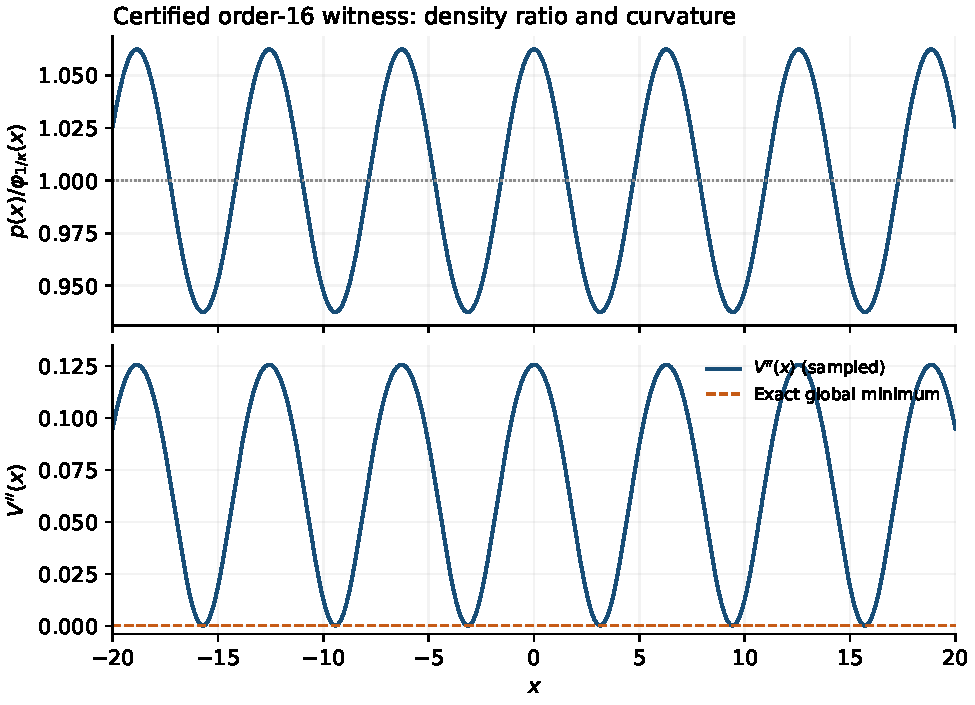
\includegraphics[width=.85\textwidth]{witness16.pdf}
\caption{The order-sixteen density relative to its Gaussian envelope, and the
curvature of its potential. The plot is illustrative; the curvature bound and the
sign of $S_{16}$ are established by the certificates.}
\end{figure}

\begin{table}[htbp]
\centering
\begin{tabular}{rrc}
\toprule
$m$ & $S_m(p_{16})$ (rounded) & sign \\
\midrule
6 & $0.0058218676$ & $+$\\
7 & $0.010328902$ & $+$\\
8 & $0.019558949$ & $+$\\
9 & $0.039284423$ & $+$\\
10 & $0.083136420$ & $+$\\
11 & $0.18369755$ & $+$\\
12 & $0.41753255$ & $+$\\
13 & $0.9490475$ & $+$\\
14 & $2.0231416$ & $+$\\
15 & $3.2947621$ & $+$\\
16 & $-0.76971251$ & $-$\\
17 & $-36.171892$ & $-$\\
18 & $-31.18273$ & $-$\\
19 & $3700.7193$ & $+$\\
20 & $75350.4$ & $+$\\
\bottomrule
\end{tabular}
\caption{Entropy derivatives of $p_{16}$. Every sign is certified by a rigorous Arb
enclosure (second method of Proposition~\ref{prop:witness}); values are rounded
midpoints. Enclosures: \texttt{certs/witness\_order\_table\_paired15/}. The density
fails exactly at orders 16--18 among those listed.}
\label{tab:witness}
\end{table}

\begin{remark}[A two-mode witness at order seventeen]
The two-mode density $p\propto e^{-x^2/36}(1+\cos x/20+\cos2x/100000)$ satisfies
$(-\log p)''>1/400$ and $S_{17}(p)<-3/20$, with two independent enclosures
(Appendix~\ref{app:series} and a spatial computation) whose enclosures overlap.
Numerically, two-mode families of this type do not reach order sixteen; the third
mode is what lowers the threshold by one.
\end{remark}

\section{The Zou--Fan--Gao--Wang family at finite order}\label{sec:zou}
Zou, Fan, Gao and Wang~\cite{ZFGW26} prove that $f_m$ (Theorem~\ref{thm:zou})
violates the sign condition for all sufficiently large $m$, with
$(-1)^mH^{(m)}_{f_m}(0)=-\tfrac{11}{96}\beta^m+o(\beta^m)$, $\beta=3/(2\sqrt2)$, but
without an explicit threshold.

\begin{proposition}\label{prop:zou}
For each $6\le M\le400$, the rigorous enclosure of Appendix~\ref{app:series}, applied
to the member $f_M$ at its own order $M$ with $a_M=2^{-M/4}$ enclosed in an Arb ball,
$b_M=2^{-M}$ exact and $\kappa_M=8a_M$, gives $S_M(f_M)>0$ for $6\le M\le32$ and
$S_M(f_M)<0$ for $33\le M\le400$.
\end{proposition}
Every admissibility condition of Appendix~\ref{app:series} ($|a|+|b|<1$, $\kappa>0$
and a positive curvature bound) is decided rigorously on the balls. All $395$ members
were resolved with series cutoff $N=160$, Fourier cutoff $K=16$ and $120$ digits; the
whole computation takes about three and a half minutes on one CPU core. For $M=32,33,36$
the signs were also confirmed with the heat-evolution method of
Proposition~\ref{prop:witness} (\texttt{src/zou\_crosscheck.py}; for $M=33$ with a
rational $a_{33}$ within relative distance $10^{-30}$ of $2^{-33/4}$), the enclosures
agreeing to at least twelve digits. The enclosures are in
\texttt{checkpoints/zou\_family\_threshold.json} and
\texttt{checkpoints/zou\_crosscheck.json}. The family's first failing order,
thirty-three, is seventeen above that of $p_{16}$.

\section{A family with exponential tails}\label{sec:logcosh}
\begin{proposition}
For $p_{\alpha,\beta}(x)\propto e^{\beta x}\cosh(x)^{-\alpha}$ with $\alpha>0$ and
$|\beta|<\alpha$, one has $S_m(p_{\alpha,\beta})>0$ for every $2\le m\le17$.
\end{proposition}
\begin{proof}
Here $V''=\alpha\operatorname{sech}^2x>0$, all higher log-derivatives are bounded, and
exponential tails justify the differentiation. Put $T=\tanh X$; then $(1+T)/2$ is
beta-distributed with parameters $(\alpha\pm\beta)/2$, and the moments $M_k=\E T^k$
satisfy $M_0=1$, $M_1=\beta/\alpha$, $M_{k+1}=(\beta M_k+kM_{k-1})/(\alpha+k)$. The
score derivatives of order at least two are $\alpha$ times polynomials in $T$.
Substituting into the entropy recurrence, multiplying by
$(\alpha)_{2m}=\prod_{j<2m}(\alpha+j)$ and setting $s=1-\beta^2/\alpha^2\in(0,1]$
gives $(\alpha)_{2m}S_m=\sum_i\alpha^i\sum_kb_{m,i,k}\binom{n_i}ks^k(1-s)^{n_i-k}$
with exact rational $b_{m,i,k}\ge0$ and, for each $m$, a strictly positive endpoint
coefficient; an independent verifier checks every identity and sign exactly.
\end{proof}
This concerns this family only and does not improve the lower bound for $m^*$.

\section{Discussion: the orders fourteen and fifteen}\label{sec:discussion}
The remaining question is whether $m^*$ equals $14$, $15$ or $16$. By
Lemma~\ref{lem:propagation}, an order-$15$ certificate alone would prove $m^*=16$.

\emph{Certificates.} The certificate SDPs grow quickly: at order 14 the quotient
system has 708 independent constraints and Gram blocks of sizes 135 and 101; at
order 15, 1039 constraints and blocks of sizes 176 and 135. Double-precision
interior-point and first-order solvers stall on these instances, and a failed solve
says nothing about existence. Moreover the ansatz~\eqref{eq:cert}, with a fixed
monomial degree and the single multiplier $-u_2$, is only a sufficient condition:
$S_{14}\ge0$ or $S_{15}\ge0$ could hold for every log-concave density without a
certificate of this form. Neither order is settled.

\emph{Numerical evidence (not proof).} For densities $e^{-\kappa x^2/2}r(x)$ with
trigonometric $r$, the exact heat evolution reduces $S_m$, up to Gaussian-filter
terms of size $e^{-1/(2\kappa)}$, to $\tfrac12(m-1)!\kappa^m$ plus a sum over
Fourier ``energy levels'' $d$ of the periodic part, each weighted by a positive
kernel. Negativity requires a negative level, such as the cubic term
$-\tfrac18a_1^2a_2$, to outweigh the positive level $\tfrac14a_1^2$, whose weight
is fixed by the log-concavity constraint $\kappa\ge\max(\log r)''$. Searches over
several families (cosine sums with up to eight modes, incommensurate frequencies,
localized wave packets on non-Gaussian convex bases, and piecewise-linear
log-densities at positive time) found no density with $S_{15}<0$; the closest
reached about $95\%$ of the curvature margin required. This is consistent with, but
does not prove, the conjecture $m^*=16$.

\section*{Data and code availability}
All certificates, verification programs and data are at \repo{} (code under the MIT
licence; text, certificates and data under CC~BY~4.0). The README lists the commands
that reproduce every verification on a CPU; \texttt{requirements-verify.txt} lists
the only dependency beyond the Python standard library (\texttt{python-flint}). The
verifiers raise explicit errors and are equally strict under \texttt{python -O}. The
SHA-256 manifest \texttt{certs/exact\_certificate\_sha256.json}, checked by
\texttt{src/check\_hashes.py}, covers every certificate and enclosure cited here. The
unedited records of the automated research runs are in
\texttt{archive/process-records/}.

\section*{Use of AI}
This work was carried out with AI systems doing most of the technical work.
Anthropic's Claude models, run through Claude Code (including long autonomous runs
coordinated by a Claude model), proposed the computational strategy, wrote and ran all
of the software (symbolic derivations, numerical searches, semidefinite solvers, exact
rational reconstruction and the interval-arithmetic certifiers), found the certificates
and the counterexamples, and drafted the mathematical arguments and the text. The
revisions for version 0.2.0 were also made with Claude Code. The author posed the
question, directed and supervised the work, and reviewed the results. All certificates
and enclosures are checked by the exact rational and interval-arithmetic verifiers
released with the paper; the analytic arguments of Sections~\ref{sec:positive-time}--\ref{sec:sharp-proof}
are written proofs that have not yet been independently checked by a human expert.
The unedited records of the automated runs are archived with the code. The author
takes full responsibility for the content.

\appendix
\section{Reduced integrands}\label{app:formulas}
With $u_j=\partial_x^j\log p$, the reduced integrands of
Proposition~\ref{prop:recurrence} at orders six to eight are listed below
(generated by \texttt{src/derive\_integrands.py}; the representative is not unique
modulo integration by parts). They satisfy $\partial_t^mH(P_tp)|_{t=0}=\E_pF_m$, so
$S_m=(-1)^m\E_pF_m$; for a Gaussian of variance $v$ only the $u_2^m$ term survives,
giving $S_m=(m-1)!/(2v^m)$.
{\small
\begin{align*}
F_{6}={}&\frac{u_{6}^{2}}{2} -15 u_{4}^{3} +60 u_{2}^{6} +105 u_{3}^{4}\\
&{}-600 u_{2}^{3} u_{3}^{2} -15 u_{2} u_{5}^{2} +150 u_{2}^{2} u_{4}^{2} -60 u_{3} u_{4} u_{5}\\
&{}+450 u_{2} u_{3}^{2} u_{4}
\end{align*}
\begin{align*}
F_{7}={}&360 u_{2}^{7} -\frac{u_{7}^{2}}{2} -6300 u_{2}^{4} u_{3}^{2} -2415 u_{3}^{2} u_{4}^{2}\\
&{}-630 u_{2} u_{4}^{3} -630 u_{3}^{3} u_{5} -315 u_{2}^{2} u_{5}^{2} +21 u_{2} u_{6}^{2}\\
&{}+70 u_{4}^{2} u_{6} +105 u_{4} u_{5}^{2} +2100 u_{2}^{3} u_{4}^{2} +4410 u_{2} u_{3}^{4}\\
&{}+105 u_{3} u_{5} u_{6} +9450 u_{2}^{2} u_{3}^{2} u_{4} -2520 u_{2} u_{3} u_{4} u_{5}
\end{align*}
\begin{align*}
F_{8}={}&\frac{u_{8}^{2}}{2} +2520 u_{2}^{8} +3115 u_{4}^{4} -70560 u_{2}^{5} u_{3}^{2}\\
&{}-47880 u_{3}^{4} u_{4} -17640 u_{2}^{2} u_{4}^{3} -5880 u_{2}^{3} u_{5}^{2} -280 u_{5}^{2} u_{6}\\
&{}-210 u_{4} u_{6}^{2} -28 u_{2} u_{7}^{2} +588 u_{2}^{2} u_{6}^{2} +7140 u_{3}^{2} u_{5}^{2}\\
&{}+29400 u_{2}^{4} u_{4}^{2} +123480 u_{2}^{2} u_{3}^{4} -135240 u_{2} u_{3}^{2} u_{4}^{2} -35280 u_{2} u_{3}^{3} u_{5}\\
&{}-280 u_{4} u_{5} u_{7} -168 u_{3} u_{6} u_{7} +3920 u_{2} u_{4}^{2} u_{6} +5880 u_{2} u_{4} u_{5}^{2}\\
&{}+5880 u_{3}^{2} u_{4} u_{6} +20160 u_{3} u_{4}^{2} u_{5} +176400 u_{2}^{3} u_{3}^{2} u_{4} -70560 u_{2}^{2} u_{3} u_{4} u_{5}\\
&{}+5880 u_{2} u_{3} u_{5} u_{6}
\end{align*}
}

\section{Rigorous Fourier-series enclosure}\label{app:series}
For $p\propto e^{-\kappa x^2/2}(1+a\cos x+b\cos2x)$, set $d=1+\kappa t$,
$\tau=t/d$ and $r(\tau,y)=1+ae^{-\tau/2}\cos y+be^{-2\tau}\cos2y$. Expand
$(1+u)\log(1+u)=u+\sum_{n\ge2}\frac{(-1)^n}{n(n-1)}u^n$. A term $a^pb^q$ with
$p+q=n$ has time exponent $L=(p+4q)/2$; Gaussian averaging of Fourier mode $k$
multiplies it by $e^{-k^2/(2\kappa)}e^{-(L-k^2/2)\tau}$. The signed order-$m$ time
derivative of $e^{-B\tau(t)}$ is the exact polynomial
\[
 T_m(B,\kappa)=\sum_{j=0}^{m-1}\frac{m!}{(m-j)!}\binom{m-1}{j}\kappa^jB^{m-j},
\]
and the zero-mode coefficient of $\cos^py\cos^q2y$ is
$2^{-n}\sum_{j}\binom qj\binom p{(p+2q-4j)/2}$ (zero for odd $p$). With
$r_0=|a|+|b|$, the degree-$n$ contributions are bounded by $r_0^n(2n+m\kappa)^m$;
after truncation at $N$ the tail is at most
\[
 \frac{(2+m\kappa)^mr_0^{N+1}(N+1)^m}{1-r_0(1+1/(N+1))^m}
\]
when the denominator is positive, and omitting Fourier modes $|k|>K$ costs at most
$e^{-y_0/\kappa}(2N+y_0+m\kappa)^m\,r_0^2/(1-r_0)$, $y_0=(K+1)^2/2$. With
$\Xi=1+ae^{-1/(2\kappa)}+be^{-2/\kappa}$ the result is
$\tfrac12(m-1)!\kappa^m+(\text{finite sum}+M_m)/\Xi$, where
$M_m=m!\kappa^{m-1}(\tfrac a2e^{-1/(2\kappa)}+2be^{-2/\kappa})$, with both error
bounds divided by $\Xi$. All arithmetic is outward-rounded Arb at 100--200 digits.
Implementation: \texttt{src/certify\_fourier\_series.py}.

\begin{thebibliography}{99}
\bibitem{ChengGeng15} F.~Cheng and Y.~Geng, Higher order derivatives in Costa's
entropy power inequality, \emph{IEEE Trans.\ Inform.\ Theory} \textbf{61} (2015),
no.~11, 5892--5905.
\bibitem{Costa85} M.~H.~M.~Costa, A new entropy power inequality,
\emph{IEEE Trans.\ Inform.\ Theory} \textbf{31} (1985), no.~6, 751--760.
\bibitem{GuSellke26} Y.~Gu and M.~Sellke, A counterexample to the Gaussian completely
monotone conjecture, arXiv:2605.11656 (2026).
\bibitem{Johansson17} F.~Johansson, Arb: efficient arbitrary-precision
midpoint-radius interval arithmetic, \emph{IEEE Trans.\ Comput.} \textbf{66} (2017),
no.~8, 1281--1292.
\bibitem{McKean66} H.~P.~McKean, Jr., Speed of approach to equilibrium for Kac's
caricature of a Maxwellian gas, \emph{Arch.\ Rational Mech.\ Anal.} \textbf{21}
(1966), 343--367.
\bibitem{Parrilo03} P.~A.~Parrilo, Semidefinite programming relaxations for
semialgebraic problems, \emph{Math.\ Program.} \textbf{96} (2003), 293--320.
\bibitem{PeyrlParrilo08} H.~Peyrl and P.~A.~Parrilo, Computing sum of squares
decompositions with rational coefficients, \emph{Theoret.\ Comput.\ Sci.}
\textbf{409} (2008), 269--281.
\bibitem{SDPA03} M.~Yamashita, K.~Fujisawa and M.~Kojima, Implementation and
evaluation of SDPA~6.0 (SemiDefinite Programming Algorithm~6.0),
\emph{Optim.\ Methods Softw.} \textbf{18} (2003), 491--505.
\bibitem{Stam59} A.~J.~Stam, Some inequalities satisfied by the quantities of
information of Fisher and Shannon, \emph{Inform.\ Control} \textbf{2} (1959), 101--112.
\bibitem{GYG22} L.~Guo, C.-M.~Yuan and X.-S.~Gao, Lower bounds on multivariate
higher order derivatives of differential entropy, \emph{Entropy} \textbf{24} (2022),
no.~8, 1155.
\bibitem{LV07} L.~Lov\'asz and S.~Vempala, The geometry of logconcave functions and
sampling algorithms, \emph{Random Structures Algorithms} \textbf{30} (2007), no.~3,
307--358.
\bibitem{SW14} A.~Saumard and J.~A.~Wellner, Log-concavity and strong
log-concavity: a review, \emph{Stat.\ Surv.} \textbf{8} (2014), 45--114.
\bibitem{Wang24} G.~Wang, A higher-order Otto calculus approach to the Gaussian
completely monotone conjecture, \emph{IEEE Trans.\ Inform.\ Theory} \textbf{71}
(2025), no.~12, 9135--9162; arXiv:2408.13957.
\bibitem{ZAG18} X.~Zhang, V.~Anantharam and Y.~Geng, Gaussian optimality for
derivatives of differential entropy using linear matrix inequalities,
\emph{Entropy} \textbf{20} (2018), no.~3, 182.
\bibitem{ZFGW26} J.~Zou, L.~Fan, J.~Gao and J.~Wang, An explicit family of
log-concave counterexamples to the Gaussian completely monotone conjecture,
arXiv:2608.30275 (2026).
\bibitem{ZFGW26hex} J.~Zou, L.~Fan, J.~Gao and J.~Wang, A hexagonal counterexample to
log-convexity of Fisher information along the heat flow, arXiv:2605.18081 (2026).
\end{thebibliography}
\end{document}
